\documentclass[10pt]{article}

\usepackage[italian]{babel}
\usepackage{caption}
\usepackage{float}
\usepackage{fullpage}
\usepackage{graphicx}
\usepackage[colorlinks=true, urlcolor=blue]{hyperref}
\usepackage[utf8]{inputenc}
\usepackage{minted}
\usepackage{subcaption}

\title{Progetto del corso Sistemi Distribuiti: Paradigmi e Modelli}
\author{
	Jacopo Notarstefano\\
	\texttt{jacopo [dot] notarstefano [at] gmail.com}
}
\date{}

% http://tex.stackexchange.com/a/4304/10806
\newcommand{\cpp}{C\nolinebreak\hspace{-.05em}\raisebox{.4ex}{\tiny\bf +}\nolinebreak\hspace{-.10em}\raisebox{.4ex}{\tiny\bf +}}

\newcommand{\mpp}{Magick\nolinebreak\hspace{-.05em}\raisebox{.4ex}{\tiny\bf +}\nolinebreak\hspace{-.10em}\raisebox{.4ex}{\tiny\bf +}}

\begin{document}
  \maketitle
    \section{Introduzione}

    Scopo di questo progetto è dare un'implementazione sequenziale e una
    parallela di una soluzione al problema dell'Histogram Thresholding, per
    poi confrontarne le performance sia fra esse sia con i modelli teorici.

    Entrambe le implementazioni sono realizzate in \cpp; in particolare
    quella parallela è data in termini di parallel skeleton, più nello
    specifico quelli forniti dal framework 
    \href{http://sketo.ipl-lab.org/}{\underline{SkeTo}}.

    SkeTo è uno skeleton framework per certi versi atipico: dichiarazione e
    istanziazione degli skeleton avvengono allo stesso tempo. I metodi
    offerti dalle classi astratte del framework, implementate in termini di
    template, sono quelli tipici della programmazione funzionale, come
    \texttt{map}, \texttt{reduce} e \texttt{scan}. Queste caratteristiche
    rendono molto compatto il codice: in effetti l'intero codice non
    funzionale parallelo di \texttt{src/parallel.cpp} ammonta a \(63\) righe 
    commenti inclusi, di cui appena \(3\) chiamate di libreria.

    \section{Il problema dell'Histogram Thresholding}

    Siano \texttt{I} un'immagine e \texttt{p} una percentuale. Supponiamo di 
    avere accesso ai singoli pixel dell'immagine, e denotiamo con 
    \texttt{I[i][j]} il pixel alla riga \texttt{i} e colonna \texttt{j}.
    Il problema dell'Histogram Thresholding consiste nel restituire
    un'immagine in bianco e nero \texttt{BW} tale che il pixel
    \texttt{BW[i][j]} sia bianco se il pixel \texttt{I[i][j]} è più luminoso
    di \texttt{p\%} pixel dell'immagine originaria, nero altrimenti.

    Osserviamo che in letteratura esistono più definizioni di luminosità di 
    un pixel; le soluzioni proposte usano la coordinata \texttt{L} nello 
    spazio colori \texttt{HSL}.

    \section{Descrizione delle implementazioni}

    Abbiamo posto particolare enfasi nella divisione fra codice funzionale e
    non funzionale; in particolare il business code dell'applicazione è
    interamente astratto nella classe \texttt{Job}, di cui diamo di seguito
    l'interfaccia:

    \inputminted[]{c++}{src/job.h}

    Osserviamo che i metodi \texttt{execute} e \texttt{writeResult} hanno
    come tipo di ritorno \texttt{Job}; in effetti questi metodi ritornano
    l'oggetto stesso. Ciò consente di usarli in \texttt{sequential.cpp} come
    se avessere tipo di ritorno \texttt{void}, e in \texttt{parallel.cpp},
    come argomento di \texttt{generate} e \texttt{map}, dopo averli astratti 
    in opportuni function object.

    La lettura e scrittura delle immagini è interamente delegata alla
    libreria \href{http://www.imagemagick.org/script/index.php}{\underline{ImageMagick}},
    tramite \href{http://www.imagemagick.org/script/magick++.php}{\underline{\mpp}},
    la sua API per \cpp.

    \section{Valutazione delle performance}

    \section{Valutazione dei risultati}

    L'algoritmo implementato nel file \texttt{src/job.cpp} produce i
    seguenti risultati al variare della soglia \texttt{p}:

    \begin{figure}[H]
      \centering
      \begin{subfigure}[b]{0.33\textwidth}
        \centering
        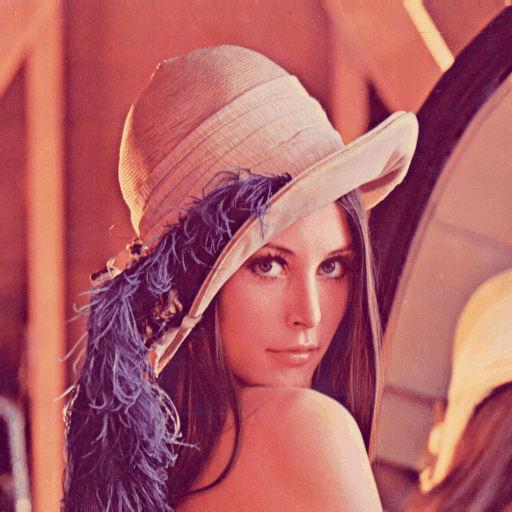
\includegraphics[width=\textwidth]{tex/img/lena.png}
        \caption*{Originale}
      \end{subfigure}
      \hspace{0.2\textwidth}
      \begin{subfigure}[b]{0.33\textwidth}
        \centering
        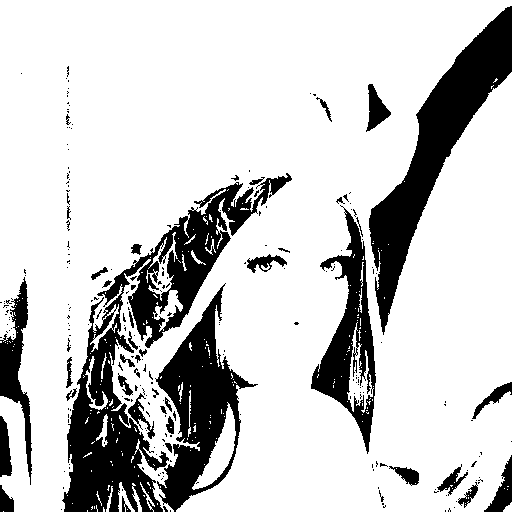
\includegraphics[width=\textwidth]{img/lena-threshold-20.png}
        \caption*{\texttt{p }\( = 20\)}
      \end{subfigure}

      \vspace{0.02\textwidth}

      \begin{subfigure}[b]{0.33\textwidth}
        \centering
        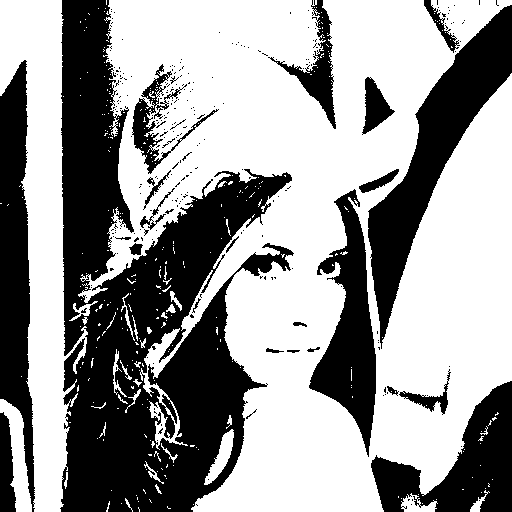
\includegraphics[width=\textwidth]{img/lena-threshold-40.png}
        \caption*{\texttt{p }\( = 40\)}
      \end{subfigure}
      \hspace{0.2\textwidth}
      \begin{subfigure}[b]{0.33\textwidth}
        \centering
        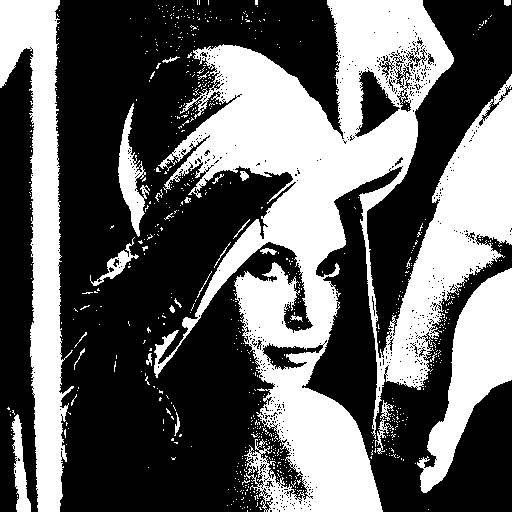
\includegraphics[width=\textwidth]{img/lena-threshold-60.png}
        \caption*{\texttt{p }\( = 60\)}
      \end{subfigure}

      \vspace{0.02\textwidth}

      \begin{subfigure}[b]{0.33\textwidth}
        \centering
        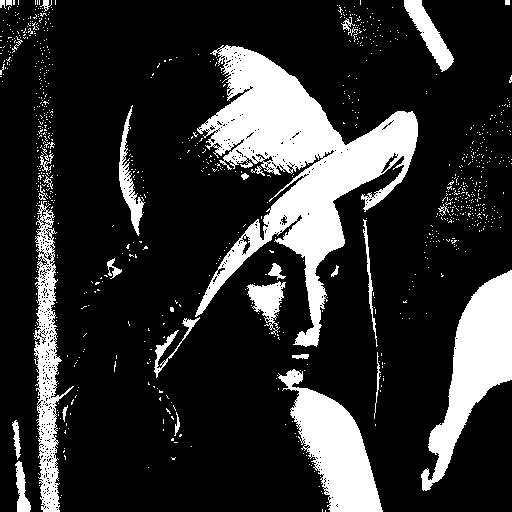
\includegraphics[width=\textwidth]{img/lena-threshold-80.png}
        \caption*{\texttt{p }\( = 80\)}
      \end{subfigure}
      \hspace{0.2\textwidth}
      \begin{subfigure}[b]{0.33\textwidth}
        \centering
        
\includegraphics[width=\textwidth]{img/lena-threshold-99.png}
        \caption*{\texttt{p }\( = 99\)}
      \end{subfigure}
    \end{figure}

    È inoltre possibile

  \appendix
    \section{Manuale d'uso}
\end{document}


































